\graphicspath{{../../S12_Notions_de_probabilites/Images/}}

\themeO
\chapter{Notions de probabilités}
\label{S12}

\programme%
   {\item Vocabulaire des probabilités.
    \item Notion de probabilités.}
   {\item Aborder les questions relatives au hasard à partir de problèmes simples.
    \item Calculer des probabilités dans des cas simples.}

\vfill

\begin{debat}{Débat : histoire des probabilités}
   C’est en cherchant à résoudre des problèmes posés par les jeux de hasard que les mathématiciens donnent naissance aux {\bf probabilités}. Lors de fouilles archéologiques, on a trouvé des indices montrant que les jeux de hasard se pratiquaient déjà 5\,000 ans av. J.-C. (on utilisait des osselets). Les premiers dés connus ont été mis à jour à {\it Tepe Gawra}, au nord de l’Irak, et datent du troisième millénaire av. J.-C. Le jeu de cartes était également pratiqué dans divers pays depuis des époques reculées. Les cartes actuelles apparaissent en France au {\small XIV}\up{e} siècle et leur utilisation donne très vite lieu à des jeux d’argent. On attribue souvent la réelle naissance à la fin du {\small XVII}\up{e} siècle ce qui en fait une branche des mathématiques relativement récente.
   \tcblower
      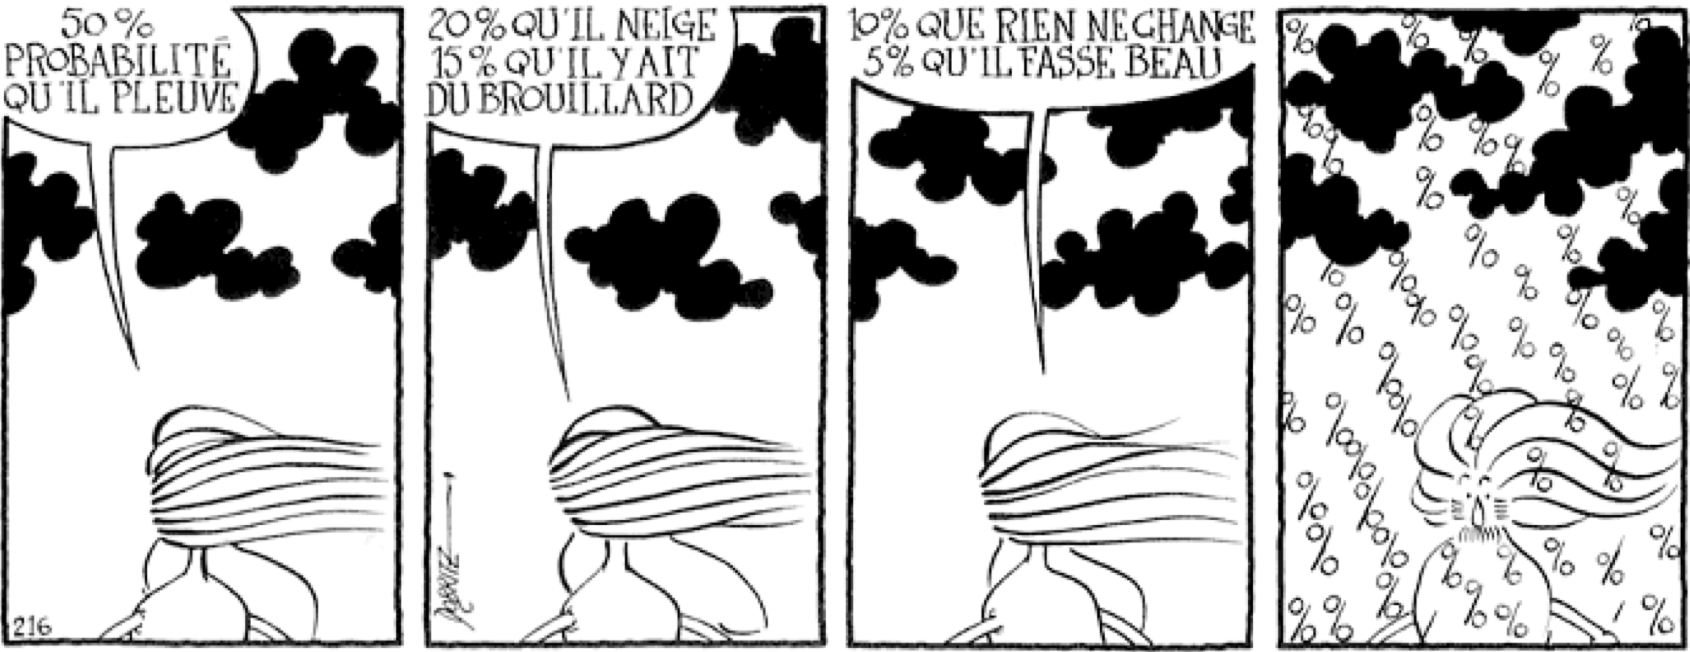
\includegraphics[width=12cm]{Dobritz} \par
      {\it Robin de l'île} par {\bf Dobritz}.
\end{debat}

\hfill {\gray Vidéo : \href{https://www.youtube.com/watch?time_continue=1&v=0xtn22h6LHE&embeds_referring_euri=https%3A%2F%2Fwww.arieka.fr%2F&source_ve_path=Mjg2NjY&feature=emb_logo}{\bf Les probabilités}, chaîne YouTube {\it Rapémathiques}, par {\it A'Rieka}.}


%%% Approche %%%
\begin{Maquette}[Cours]{Theme={Activité d'approche},Couleur={SteelBlue}}

   \AAtitre{Imposible, probable o seguro ?}

      {\it Objectifs : placer un événement sur une échelle de probabilité. }

      \begin{AActivite}

         \AApartie{Traduction}
            Traduire en français les six vignettes de cette illustration.
            \begin{center}
               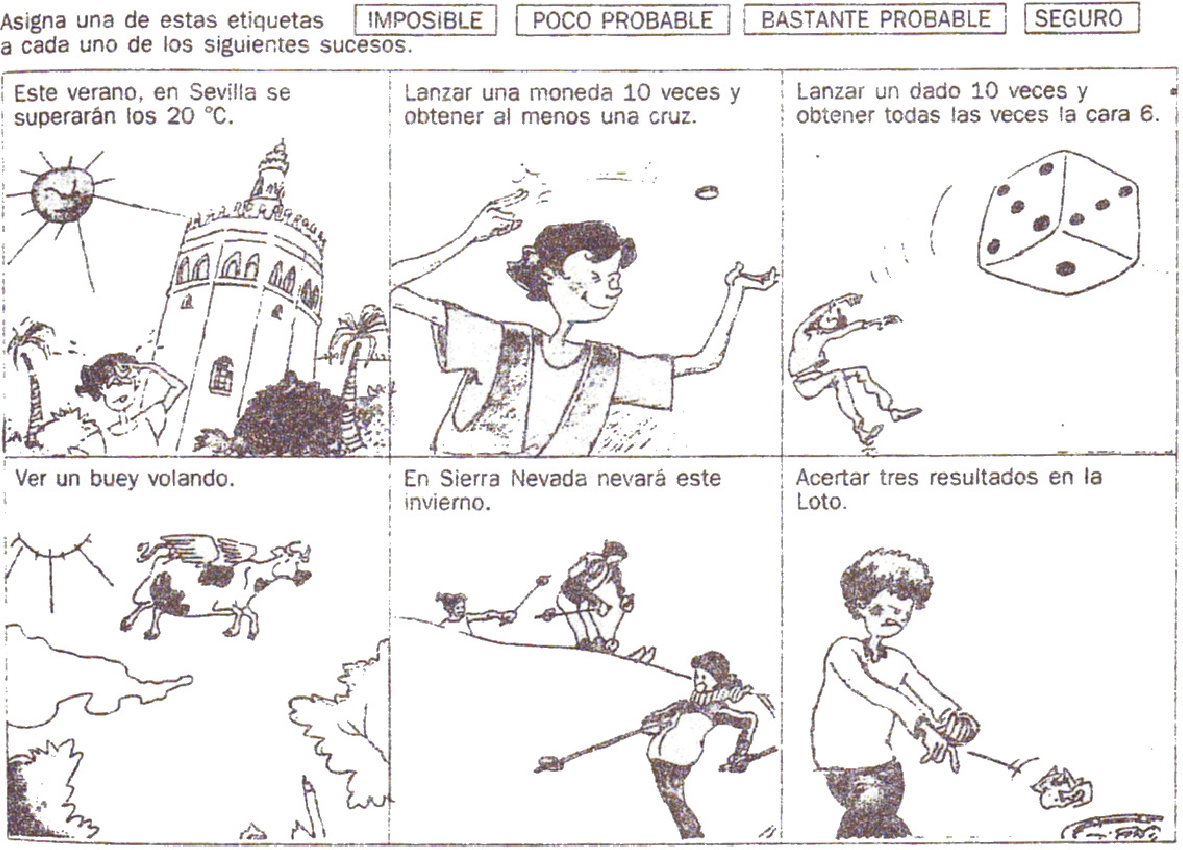
\includegraphics[width=16cm]{BD}
            \end{center}
            \begin{itemize}
               \item Vignette 1 : \pointilles
               \item Vignette 2 : \pointilles
               \item Vignette 3 : \pointilles
               \item Vignette 4 : \pointilles
               \item Vignette 5 : \pointilles
               \item Vignette 6 : \pointilles
            \end{itemize}

         \AApartie{Exploitation}
            Classer ces vignettes sur l'échelle ci-dessous en indiquant le numéro de la vignette en dessous de l'échelle.
            \begin{center}
               \begin{pspicture}(0,-1)(12,0.5)
                  \psline{->}(0,0)(12,0)
                  \footnotesize
                  \rput(0,0.3){imposible}
                  \rput(4,0.3){poco probable}
                  \rput(8,0.3){bastante probable}
                  \rput(12,0.3){seguro}
               \end{pspicture}
            \end{center}

   \end{AActivite}

   \vfill\hfill{\it\footnotesize Source : \href{https://publimath.univ-irem.fr/numerisation/RO/IRO09001/IRO09001.pdf}{\og Une initiation aux probabilités par le jeu \fg}, IREM de Rouen.}

\end{Maquette}


%%%Trace écrite %%%
\begin{Maquette}[Cours]{Theme={Trace écrite},Couleur={0.4[SteelBlue,Black]}}

   %%%1
   \section{Vocabulaire des probabilités}

      \begin{definition*}{}
         On appelle \textbf{expérience aléatoire} une expérience dont on ne peut pas prévoir le résultat de façon certaine.
      \end{definition*}

      \begin{exemple*}{}
         Lancer une pièce de monnaie est une expérience aléatoire dont le résultat est soit \og pile \fg, soit \og face \fg.
      \end{exemple*}

      \begin{definition*}{}
         \begin{itemize}
            \item Chaque résultat possible et prévisible d'une expérience aléatoire est appelé une \textbf{issue}.
            \item L'ensemble formé par les issues est appelé \textbf{univers}, souvent noté $\Omega$.
            \item Un \textbf{événement} de l'expérience aléatoire est une partie quelconque de l'univers.
         \end{itemize}
      \end{definition*}

      \begin{exemple*}{}
         \begin{itemize}
            \item Lancer d'une pièce de monnaie : $\Omega =\{$~pile~;~face~$\}$.
            \item Lancer d'un dé à six faces : $\Omega =\{~1~;~2~;~3~;~4~;~5~;~6~\}$.
            \item \og Obtenir un numéro pair \fg{} est un événement que l'on peut noter $A=\{~2~;~4~;~6~\}$.
         \end{itemize}
      \end{exemple*}


   \section{Calcul de probabilités} %%%

      La probabilité $P$ d'un événement est \og la chance \fg{} qu'il se produise.

      \begin{definition*}{}
         On dit qu'il y a \textbf{équiprobabilité} lorsque toutes les issues ont la même probabilité ; \par \smallskip
         dans ce cas, on a $P=\dfrac{\textrm{nombre d'issues favorables}}{\textrm{nombre de cas possibles}}$.
      \end{definition*}

      Remarque : dans un exercice, pour signifier que l'on est dans une situation d'équiprobabilité, on a des expressions du type : \og on lance un dé \textbf{non pipé} \fg ; \og dans une urne, les boules sont \textbf{indiscernables} au toucher \fg ; \og on rencontre \textbf{au hasard} une personne parmi\dots \fg.

      \begin{exemple*}{}
         On tire une carte dans un jeu non truqué de 52 cartes. Quelle est la probabilité d'obtenir une tête ? \par
         Le jeu est non truqué, il y a donc équiprobabilité. Les issues possibles sont le valet, la dame et le roi de pique, de carreau, de trèfle et de c\oe ur ce qui fait $4\times3$ cartes donc, $P =\dfrac{12}{52}$.
      \end{exemple*}

      \begin{propriete*}{}
         Un probabilité est toujours comprise entre 0 et 1. Si elle est égale à 0, on dit que l'événement est {\bf impossible} et si elle est égale à 1, l'événement est {\bf certain}.
      \end{propriete*}

      \begin{exemple*}{}
         On lance un dé classique équilibré à six faces. Quelle est la probabilité d'obtenir un 9 ? d'obtenir un nombre entier ? \par
         Nous sommes dans une situation d'équiprobabilité.
         \begin{itemize} 
            \item On ne peut pas obtenir un 9 avec un dé à 6 faces donc, $P =\dfrac06 =0$.
            \item Tous les nombres obtenus sont entiers donc, $P =\dfrac66 =1$.
         \end{itemize}
      \end{exemple*}

\end{Maquette}


%%% Exercices %%%
\begin{Maquette}[Fiche,CorrigeFin,Colonnes=2]{}
   
   \begin{multicols}{2}

      \begin{exercice}[SLF] %1
         Pour chacun des événements suivants, indiquer s'il relève du hasard et si oui, le placer sur l'échelle ci-dessous.
         \begin{center}
            \begin{pspicture}(0,-0.5)(7.9,0.5)
               \psline{->}(0.3,0)(7.7,0)
               \rput(4,0){|}
               \footnotesize
               \rput{90}(0.1,-0.2){impossible}
               \rput{90}(7.9,0){certain}
               \rput(1.2,0.3){improbable}
               \rput(3,0.3){peu probable}
               \rput(4.8,0.3){probable}
               \rput(6.5,0.3){très probable}
            \end{pspicture}
         \end{center}
         \begin{enumerate}
            \item Obtenir pile au jeu de pile ou face \pointilles
            \item La fête nationale aura lieu le 14 juillet \pointilles
            \item Un élève aura des baskets demain \pointilles
            \item Obtenir 6 avec un dé à six faces \pointilles
            \item Trouver la bonne combinaison au loto \pointilles
            \item Demain il fera beau \pointilles
         \end{enumerate}
      \end{exercice}
      
      \begin{Solution}
         \begin{enumerate}
            \item Obtenir pile au jeu de pile ou face : \cor{hasard}.
            \item La fête nationale aura lieu le 14 juillet.
            \item Un élève aura des baskets demain : \cor{hasard}.
            \item Obtenir 6 avec un dé à six faces : \cor{hasard}.
            \item Trouver la bonne combinaison au loto : \cor{hasard}.
            \item Demain il fera beau : \cor{hasard}.
         \end{enumerate}
         \begin{pspicture}(0,-0.9)(8,0.9)
            \psline{->}(0.3,0)(7.7,0)
            \rput(4,0){|}
            \footnotesize
            \rput{90}(0.1,0){impossible}
            \rput{90}(7.9,0){certain}
            \rput(1.2,0.3){improbable}
            \rput(3,0.3){peu probable}
            \rput(4.8,0.3){probable}
            \rput(6.5,0.3){très probable}
            \rput(5,-0.4){\cor{1}}
            \rput(7.7,-0.4){\cor{2}}
            \rput(6,-0.4){\cor{3}}
            \rput(3,-0.4){\cor{4}}
            \rput(1,-0.4){\cor{5}}
            \rput(3.9,-0.4){\cor{6}}
         \end{pspicture}
      \end{Solution}
      
      
      \begin{exercice}[SLF] %2
         Une roue de loterie est partagée en huit secteurs identiques numérotés de 1 à 8. Calculer la probabilité de chaque événement et les placer sur l'échelle.
         \begin{center}
            \begin{pspicture}(0,-0.5)(7.9,0.5)
               \psline{->}(0.3,0)(7.7,0)
               \rput(4,0){|}
               \footnotesize
               \rput{90}(0.1,-0.2){impossible}
               \rput{90}(7.9,0){certain}
               \rput(1.2,0.3){improbable}
               \rput(3,0.3){peu probable}
               \rput(4.8,0.3){probable}
               \rput(6.5,0.3){très probable}
            \end{pspicture}
         \end{center}
         \begin{enumerate}
            \item \og Obtenir 2 : \pointilles
            \item \og Obtenir un multiple de 2 : \pointilles
            \item \og Obtenir un nombre supérieur à 4 : \pointilles
            \item \og Obtenir un nombre positif : \pointilles
            \item \og Obtenir un nombre impair : \pointilles
            \item \og Obtenir un multiple de 13 : \pointilles
         \end{enumerate}
      \end{exercice}
      
      \begin{Solution}
         \begin{enumerate}
            \item Obtenir 2 : \cor{$P =1/8$}
            \item Obtenir un multiple de 2 : \cor{$P =4/8$}
            \item Obtenir un nombre supérieur à 5 : \cor{$P =3/8$}
            \item Obtenir un nombre positif : \cor{$P =8/8 =1$}
            \item Obtenir un nombre impair : \cor{$P =4/8$}
            \item Obtenir un multiple de 13 : \cor{$P =0/8 =0$}
         \end{enumerate}
         \begin{pspicture}(0,-1)(8,0.9)
            \psline{->}(0.3,0)(7.7,0)
            \rput(4,0){|}
            \footnotesize
            \rput{90}(0.1,0){impossible}
            \rput{90}(7.9,0){certain}
            \rput(1.2,0.3){improbable}
            \rput(3,0.3){peu probable}
            \rput(4.8,0.3){probable}
            \rput(6.5,0.3){très probable}
            \rput(3,-0.4){\cor{1}}
            \rput(5,-0.4){\cor{2 et 5}}
            \rput(4,-0.4){\cor{3}}
            \rput(7.5,-0.4){\cor{4}}
            \rput(0.5,-0.4){\cor{6}}
         \end{pspicture}
      \end{Solution}

       
      \begin{exercice} %3
         Roudayna tire une carte dans un jeu ordinaire de cinquante-deux cartes.
         \begin{enumerate}
            \item Donner les probabilités qu'elle obtienne les événements suivants : \og Obtenir un carreau \fg ; \og Obtenir un valet \fg{} et \og Obtenir un valet de carreau \fg.
            \item Calculer la probabilité de ne pas obtenir de carreau.
         \end{enumerate}
      \end{exercice}
      
      \begin{Solution}
         \begin{enumerate}
            \item Obtenir un carreau : $\cor{P =\dfrac{13}{52}}$. \par
               Obtenir un valet : $\cor{P =\dfrac{4}{52}}$. \par
               Obtenir un valet de carreau  : $\cor{P =\dfrac{1}{52}}$. \smallskip
            \item La probabilité de ne pas obtenir de carreau s'obtient en calculant la probabilité d'obtenir un c\oe ur, un pique ou un trèfle, ce qui fait au total $3\times13$ carte, soit 39 cartes. \cor{$P =\dfrac{39}{52}$}.
         \end{enumerate}      
      \end{Solution}
      
      
      \begin{exercice} %4
         On dispose d’un dé à six faces numérotées de 1 à 6 et d’un dé à quatre faces avec des sommets numérotés de 1 à 4, parfaitement équilibrés. On lance les deux dés.
         \begin{enumerate}
            \item Avec quel dé la probabilité d’obtenir un 3 est-elle la plus grande ?
            \item Avec quel dé la probabilité d’obtenir un multiple de 3 est-elle la plus grande ?
         \end{enumerate}
      \end{exercice}
      
      \begin{Solution}
         \begin{enumerate}
            \item Dé à six faces : $P =\dfrac16$ (obtenir 3) ; \par
               dé à quatre faces : $P =\dfrac14$ (obtenir 3). \par \smallskip
               C'est avec le \cor{dé à quatre faces} que la probabilité d'obtenir un 3 est la plus grande.
            \item Dé à six faces : $ P =\dfrac26$ (obtenir 3 ou 6) ; \par
               dé à quatre faces : $P =\dfrac14$ (obtenir 3). \par  \smallskip
               C'est avec le \cor{dé à six faces} que la probabilité d'obtenir un multiple de 3 est la plus grande.
         \end{enumerate}
      \end{Solution}
      
      
      \begin{exercice}[Dur] %5
         On écrit sur les faces d’un dé équilibré à six faces, chacune des lettres du mot : NOTOUS. On lance le dé et on regarde la lettre inscrite sur la face supérieure.
         \begin{enumerate}
            \item Quelles sont les issues de cette expérience ?
            \item Déterminer la probabilité des évènements suivants :
            \begin{enumerate}
               \item $E_1$ : \og On obtient la lettre O. \fg
               \item $E_2$ : \og On obtient une consonne. \fg
               \item $E_3$ : \og On obtient une lettre du mot KIWI. \fg
               \item $E_4$ : \og On obtient une lettre du mot CAGOUS. \fg
            \end{enumerate}
            \item Graduer un axe et y placer les probabilités des évènements précédents.
         \end{enumerate}
      \end{exercice}
      
      \begin{Solution}
         \begin{enumerate}
            \item Les issues possibles sont les lettres \cor{N, O, T, U, S}
            \item
               \begin{enumerate}
                  \item $E_1=\{\text{O}\}$ (lettre double) donc, \cor{$P(E_1) =\dfrac26$}
                  \item  $E_2=\{\text{N, T, S}\}$ donc, \cor{$P(E_2) =\dfrac36$}
                  \item  $E_3=\{\varnothing\}$ donc, \cor{$P(E_3) =\dfrac06 =0$}
                  \item  $E_4=\{\text{O, U, S}\}$ donc, \cor{$P(E_4) =\dfrac46$}
               \end{enumerate}
            \item Axe de graduation : \par
               \begin{pspicture}(0,-0.5)(8,0.9)
                  \psline{->}(0.3,0)(7.7,0)
                  \rput(4,0){|}
                  \footnotesize
                  \rput{90}(0.1,0){impossible}
                  \rput{90}(7.9,0){certain}
                  \rput(1.2,0.3){improbable}
                  \rput(3,0.3){peu probable}
                  \rput(4.8,0.3){probable}
                  \rput(6.5,0.3){très probable}
                  \rput(3.5,-0.5){\cor{$E_1$}}
                  \rput(4.5,-0.5){\cor{$E_2$}}
                  \rput(0.5,-0.5){\cor{$E_3$}}
                  \rput(5.5,-0.5){\cor{$E_4$}}
               \end{pspicture}
         \end{enumerate}
      \end{Solution}
      
      
      \begin{exercice} %6
         Trois personnes, Ali, Ben et Charles, ont chacune un sac contenant des billes. Chacune tire au hasard une bille de son sac dont le contenu est le suivant : \par \smallskip
            {\hautab{1.3}
            \begin{tabular}{|*{3}{C{2.2}|}}
               \hline
               Sac d'Ali & Sac de Ben & Sac de Charles \\
               \hline
               10 billes rouges & 97 billes rouges & 5 billes rouges \\
               30 billes noires & 3 billes noires & \\
               \hline
            \end{tabular}} \par \smallskip
         Laquelle de ces trois personnes a-t-elle la plus grande probabilité de tirer une bille rouge ? Justifier.
      \end{exercice}
      
      \begin{Solution}
         Probabilité de tirer une bille rouge :
         \begin{itemize}
            \item Pour Ali : $P =\dfrac{10}{40} =0,25$. \smallskip
            \item Pour Ben : $P =\dfrac{97}{100} =0,97$. \smallskip
            \item Pour Charles : $P =\dfrac{5}{5} =1$. \smallskip
         \end{itemize}
         \cor{Charles a la plus grande probabilité d'obtenir une bille rouge}, ce qui est logique puisqu'il n'a QUE des billes rouges.
      \end{Solution}
      
      
      \begin{exercice}[Dur] %7
         Dans les sac suivants, il y a déjà des billes noires et des billes rouges. \par
         Est-il possible d’ajouter un certain nombre (de ton choix) de billes bleues, de façon à satisfaire les indications données en dessous de chaque sac ? \par \smallskip
         \begin{minipage}{2.5cm} %cas 1
            \sac{\psdots[linewidth=1.5mm](0.5,0)(1,0)(1.25,0.5)(1,1)
               \psdots[linewidth=1.5mm,linecolor=red](0.25,0.5)(0.75,0.5)(0.5,1)}
         \end{minipage}
         \begin{minipage}{5.3cm}
            {\bf Cas n°1 :} \par
            La probabilité d'extraire \par
            une bille bleue est $\dfrac{5}{12}$.
         \end{minipage} \\
         \begin{minipage}{2.5cm} %cas 2
            \sac{\psdots[linewidth=1.5mm](0.25,0.5)(1,0)(1.25,0.5)
               \psdots[linewidth=1.5mm,linecolor=red](0.5,0)(0.75,0.5)(1,1)}
         \end{minipage}
         \begin{minipage}{5.3cm}
            {\bf Cas n°2 :} \par
            La probabilité d'extraire \par
            une bille bleue est $\dfrac{2}{5}$.
         \end{minipage} \\
         \begin{minipage}{2.5cm} %cas 3
            \sac{\psdots[linewidth=1.5mm](0.5,0)(0.75,0.5)
               \psdots[linewidth=1.5mm,linecolor=red](0.25,0.5)(0.5,1)(1,0)}
         \end{minipage}
         \begin{minipage}{5.3cm}
            {\bf Cas n°3 :} \par
            La probabilité d'extraire \par
            une bille rouge ou bleue est $\dfrac{3}{4}$.
         \end{minipage}
      \end{exercice}
      
      \begin{Solution}
         \begin{itemize}
            \item Cas n°1 : une probabilité de $\dfrac{5}{12}$ signifie que, pour 12 billes au total, 5 sont bleues. \par
               On a 7 billes, \cor{si on ajoute 5 billes bleue}, on aura bien une chance d'obtenir une bille bleue de $\dfrac{5}{12}$.
            \item Cas n°2 : une probabilité de $\dfrac{2}{5}$ signifie que, pour 5 billes au total, 2 sont bleues, ou encore que pour 10 billes, 4 sont bleues. \par
               On a 6 billes, \cor{si on ajoute 4 billes bleues}, on aura bien une chance d'obtenir une bille bleue de $\dfrac{2}{5}$.
            \item Cas n°3 : une probabilité de $\dfrac{3}{4}$ signifie que, pour 4 billes au total, 3 sont rouges ou bleues, ou encore que pour 8 billes, 6 sont rouges ou bleues. \par
               On a 3 billes rouges et 2 billes noires, \cor{si on ajoute 3 billes bleues}, on aura bien une chance d'obtenir une bille rouge ou bleue de $\dfrac{3}{4}$.
         \end{itemize}
      \end{Solution}

   \end{multicols}

\end{Maquette}


%%% Récré %%%
\begin{Maquette}[Cours]{Theme={Activité récréative},Couleur={IndianRed}}
    
   \ARtitre{Vers la loi des grands nombres\dots}

      {\hautab{2}
      \begin{enumerate}
         \item Compléter le tableau suivant : \par
            \begin{tabular}{|c|*{6}{C{1}|}}
               \hline
               Numéro sur la face visible du dé & 1 & 2 & 3 & 4 & 5 & 6 \\
               \hline
               Probabilité d'obtenir cette face (fraction) & & & & & & \\
               \hline
               Probabilité d'obtenir cette face (décimal) & & & & & & \\
               \hline
            \end{tabular} \par \bigskip
            Que remarque-t-on ? \pointilles

         \vfill

         {\bf Le travail s'effectue maintenant en binôme, vous avez à votre disposition un dé classique à six faces.}

         \vfill

         \item Lancer 10 fois le dé et noter les résultats obtenus dans le tableau suivant : \par \smallskip
            \begin{tabular}{|c|*{6}{C{1}|}}
               \hline
               Numéro sur la face visible du dé & 1 & 2 & 3 & 4 & 5 & 6 \\
               \hline
               Nombre de fois où cette face est obtenue & & & & & & \\
               \hline
               Probabilité d'obtenir cette face (fraction) & & & & & & \\
               \hline
               Probabilité d'obtenir cette face (décimal) & & & & & & \\
               \hline
            \end{tabular} \par \bigskip
            Que remarque-t-on ? \pointilles

         \vfill

         \item Lancer 100 fois le dé et noter les résultats obtenus dans le tableau suivant : \par \smallskip
            \begin{tabular}{|c|*{6}{C{1}|}}
               \hline
               Numéro sur la face visible du dé & 1 & 2 & 3 & 4 & 5 & 6 \\
               \hline
               Nombre de fois où cette face est obtenue & & & & & & \\
               \hline
               Probabilité d'obtenir cette face (fraction) & & & & & & \\
               \hline
               Probabilité d'obtenir cette face (décimal) & & & & & & \\
               \hline
            \end{tabular} \par \bigskip
            Que remarque-t-on ? \pointilles
         
         \vfill

         \item Répertorier les résultats de la classe entière et noter les résultats obtenus dans le tableau suivant : \\ [1mm]
            \begin{tabular}{|c|*{6}{C{1}|}}
               \hline
               Numéro sur la face visible du dé & 1 & 2 & 3 & 4 & 5 & 6 \\
               \hline
               Nombre de fois où cette face est obtenue & & & & & & \\
               \hline
               Probabilité d'obtenir cette face (fraction) & & & & & & \\
               \hline
               Probabilité d'obtenir cette face (décimal) & & & & & & \\
               \hline
            \end{tabular} \par \bigskip
            Que remarque-t-on ? \pointilles
      \end{enumerate}}

   
\end{Maquette}